\section{Cover Letter}
Hi, I'm Pablo Slavkin, I'm an electronic engineer from an electromechanical
tecnicitian base.\\
I've more than 15 years of experience in the electronic
industry working in a very abroad technology.\\
I'd began taking the client requirement and end with the fully working
prototype, I mean schematics, parts selection, PCB layout , bare firmware,
bootloader, RTOS, drivers, Linux embedded, device drivers, PCB batch production,
3D cases modeling in sync with PCB, and why not, some companion software like
web pages, frontend and backend services, databases, WebSocket's, python/bash
scripting and so.\\
During the dev phase I use to use a whole stack of up-to date software tools
like git, agile methodologies, unit testing, docker, GitLab/GitHub CI/CD with
custom runners and if it deserves hardware in the loop too.\\
Recently I've worked as a lead of small electronics teams with very good
results.\\
I've many years of experience in mounting PCB's at my own lab, using my own
p\&p, reflow-owen, stencils, etc. I'm very good with CNC machines, laser
cutting, and also very passionate about 3d printers, I've one of each at my lab
and use them regularly.\\
I've been working in the robot/cnc industry from the past 5 years.\\
Recently, in 2021, I've got a master's degree in embedded system from the UBA
university.\\
I'm interested in a new challenge where I'd share my expertise and knowledge and
at the same time, move my professional career much further.\\
Pablo Slavkin
%You could check my up-to-date resume \href{\linkgithubcvpdf}{here}.\\
%  \begin{figure}
%      \begin{center}
%         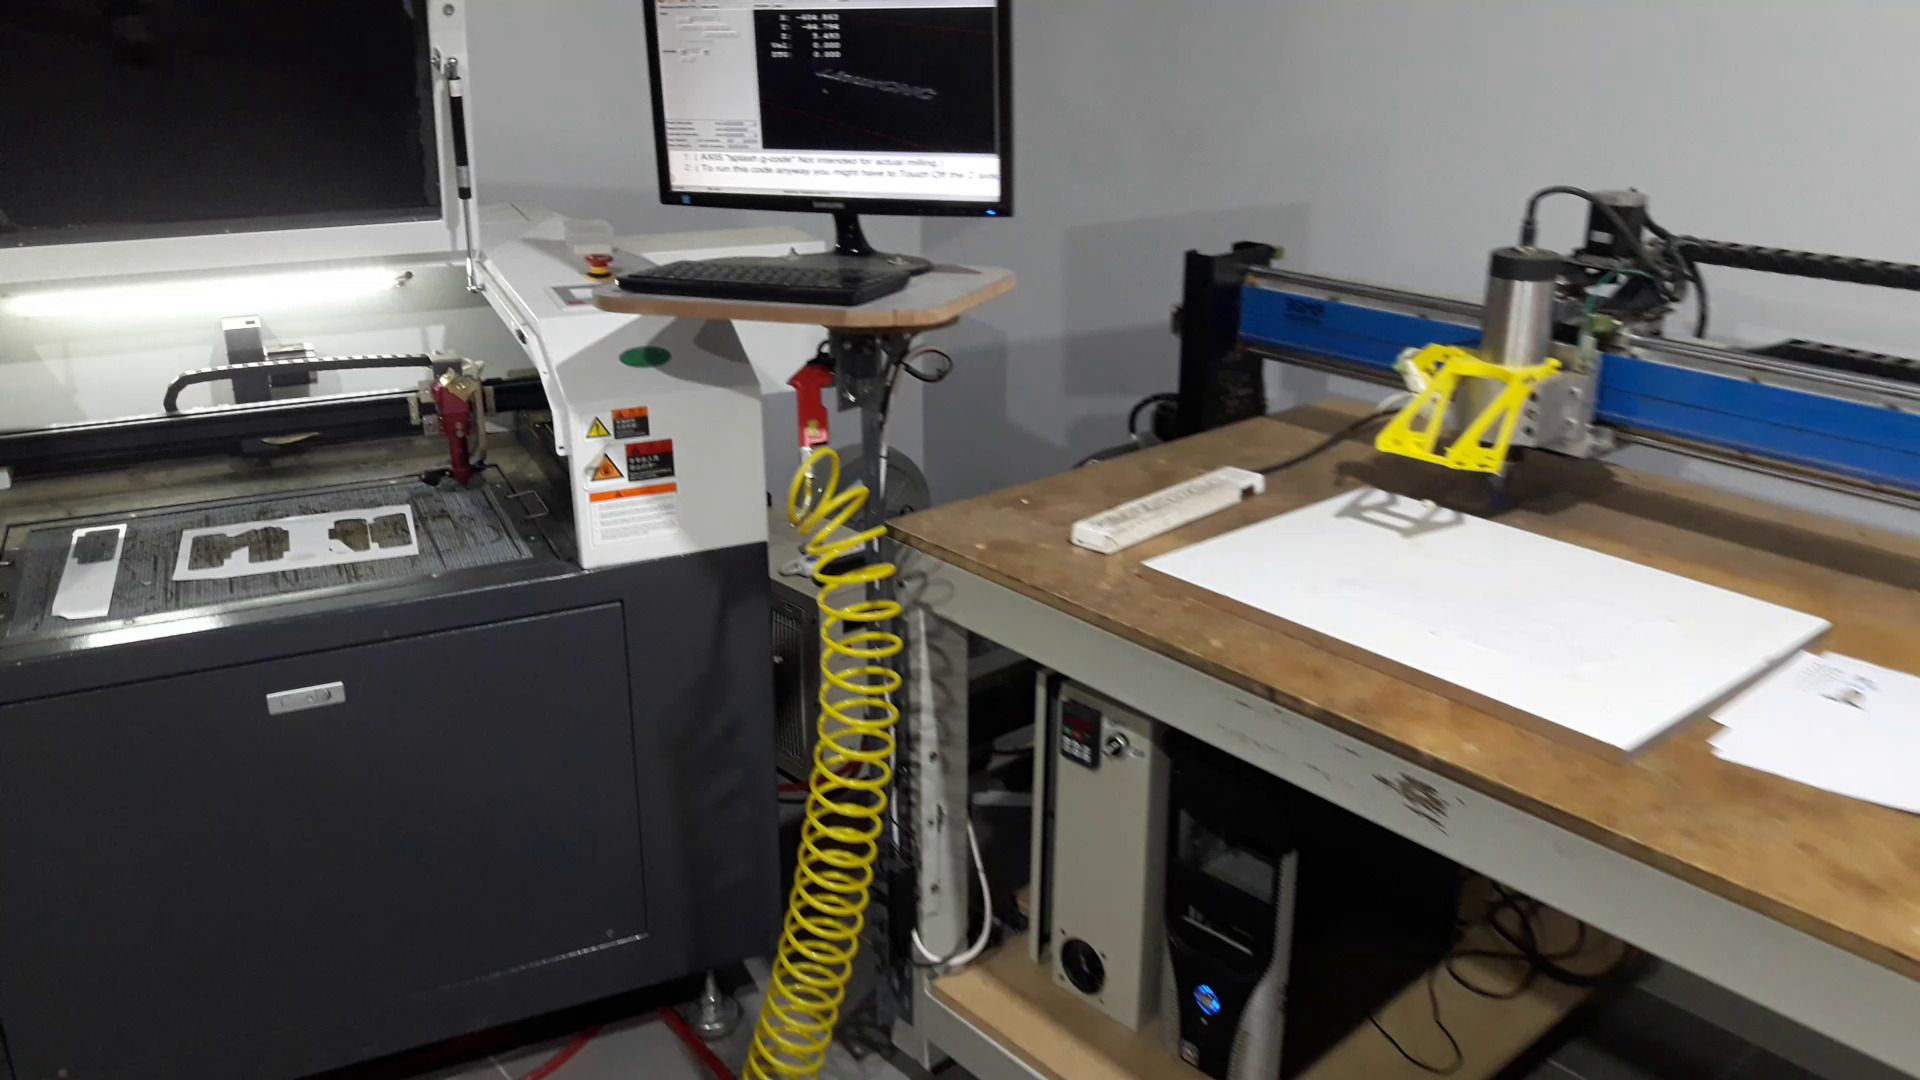
\includegraphics[width=0.3\textwidth]{ofi_dci_brc_2021_1.jpg}
%         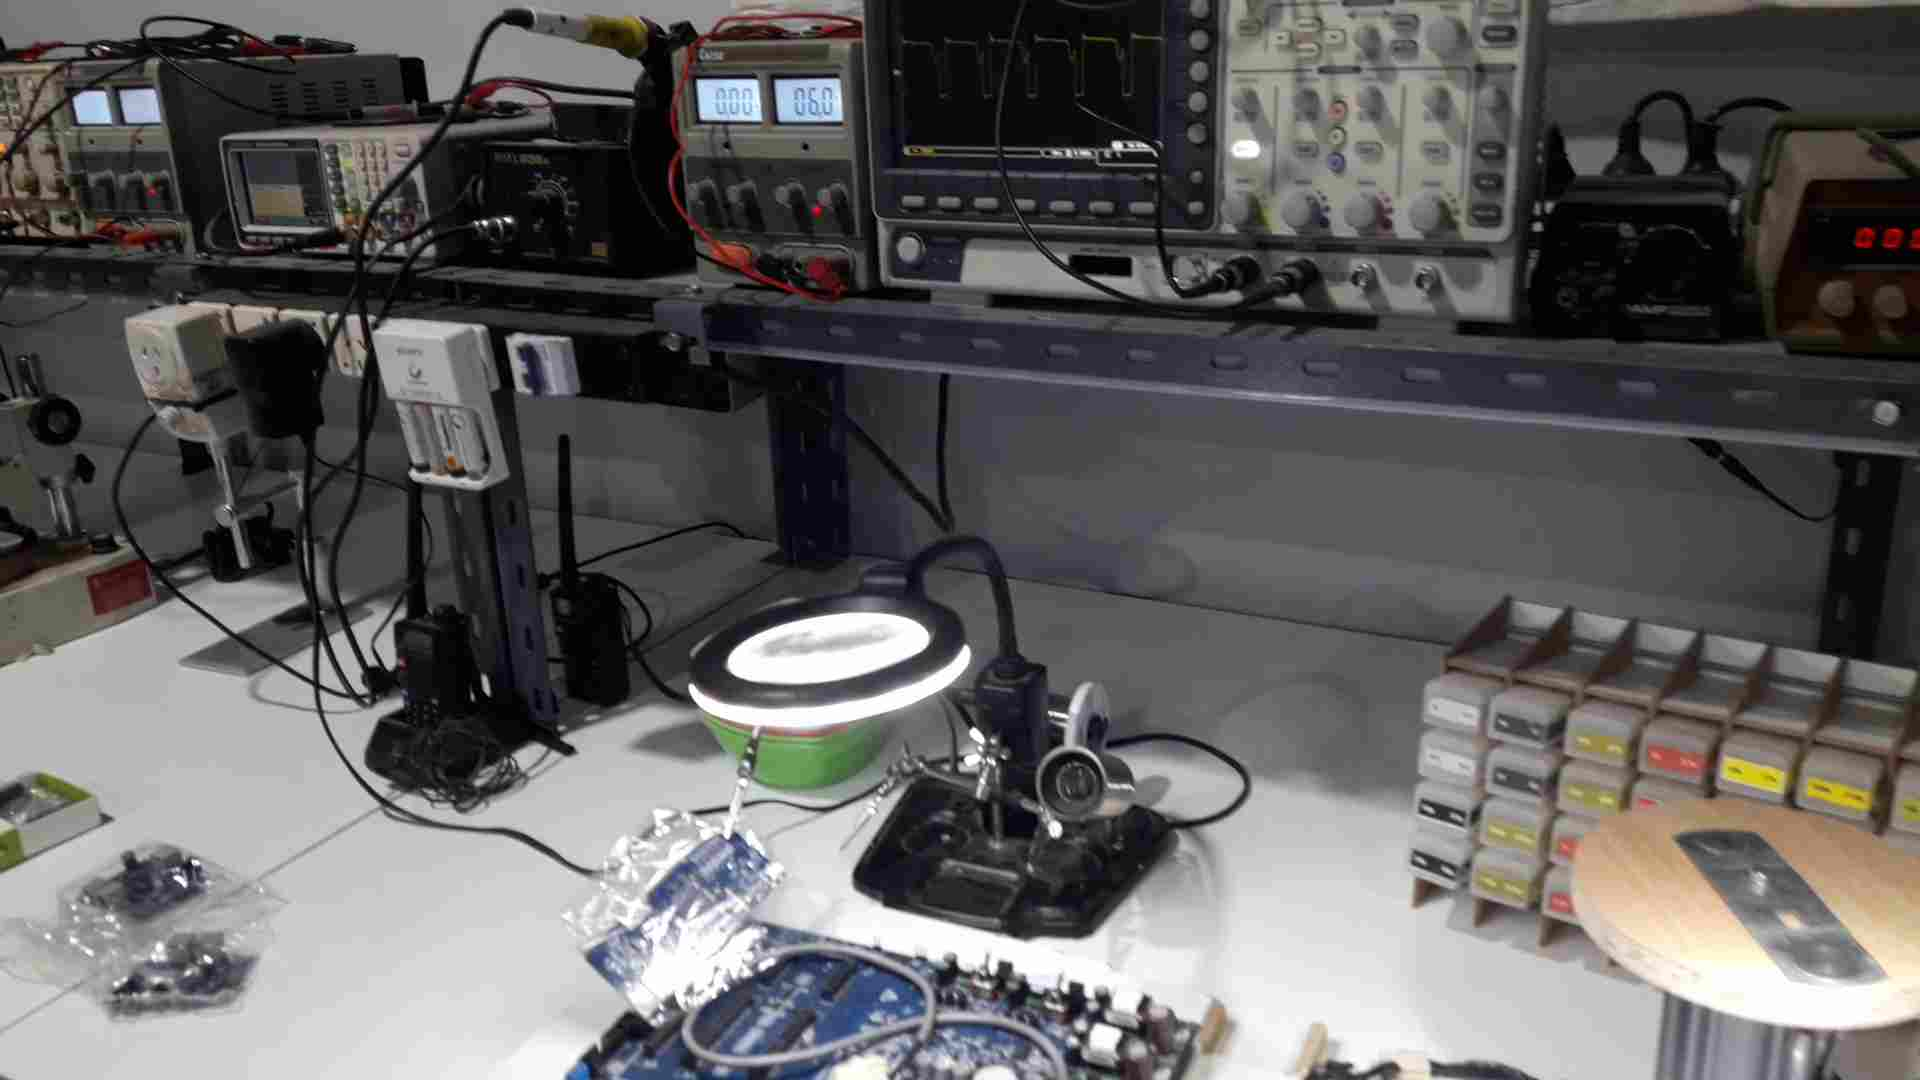
\includegraphics[width=0.3\textwidth]{ofi_dci_brc_2021_2.jpg}
%         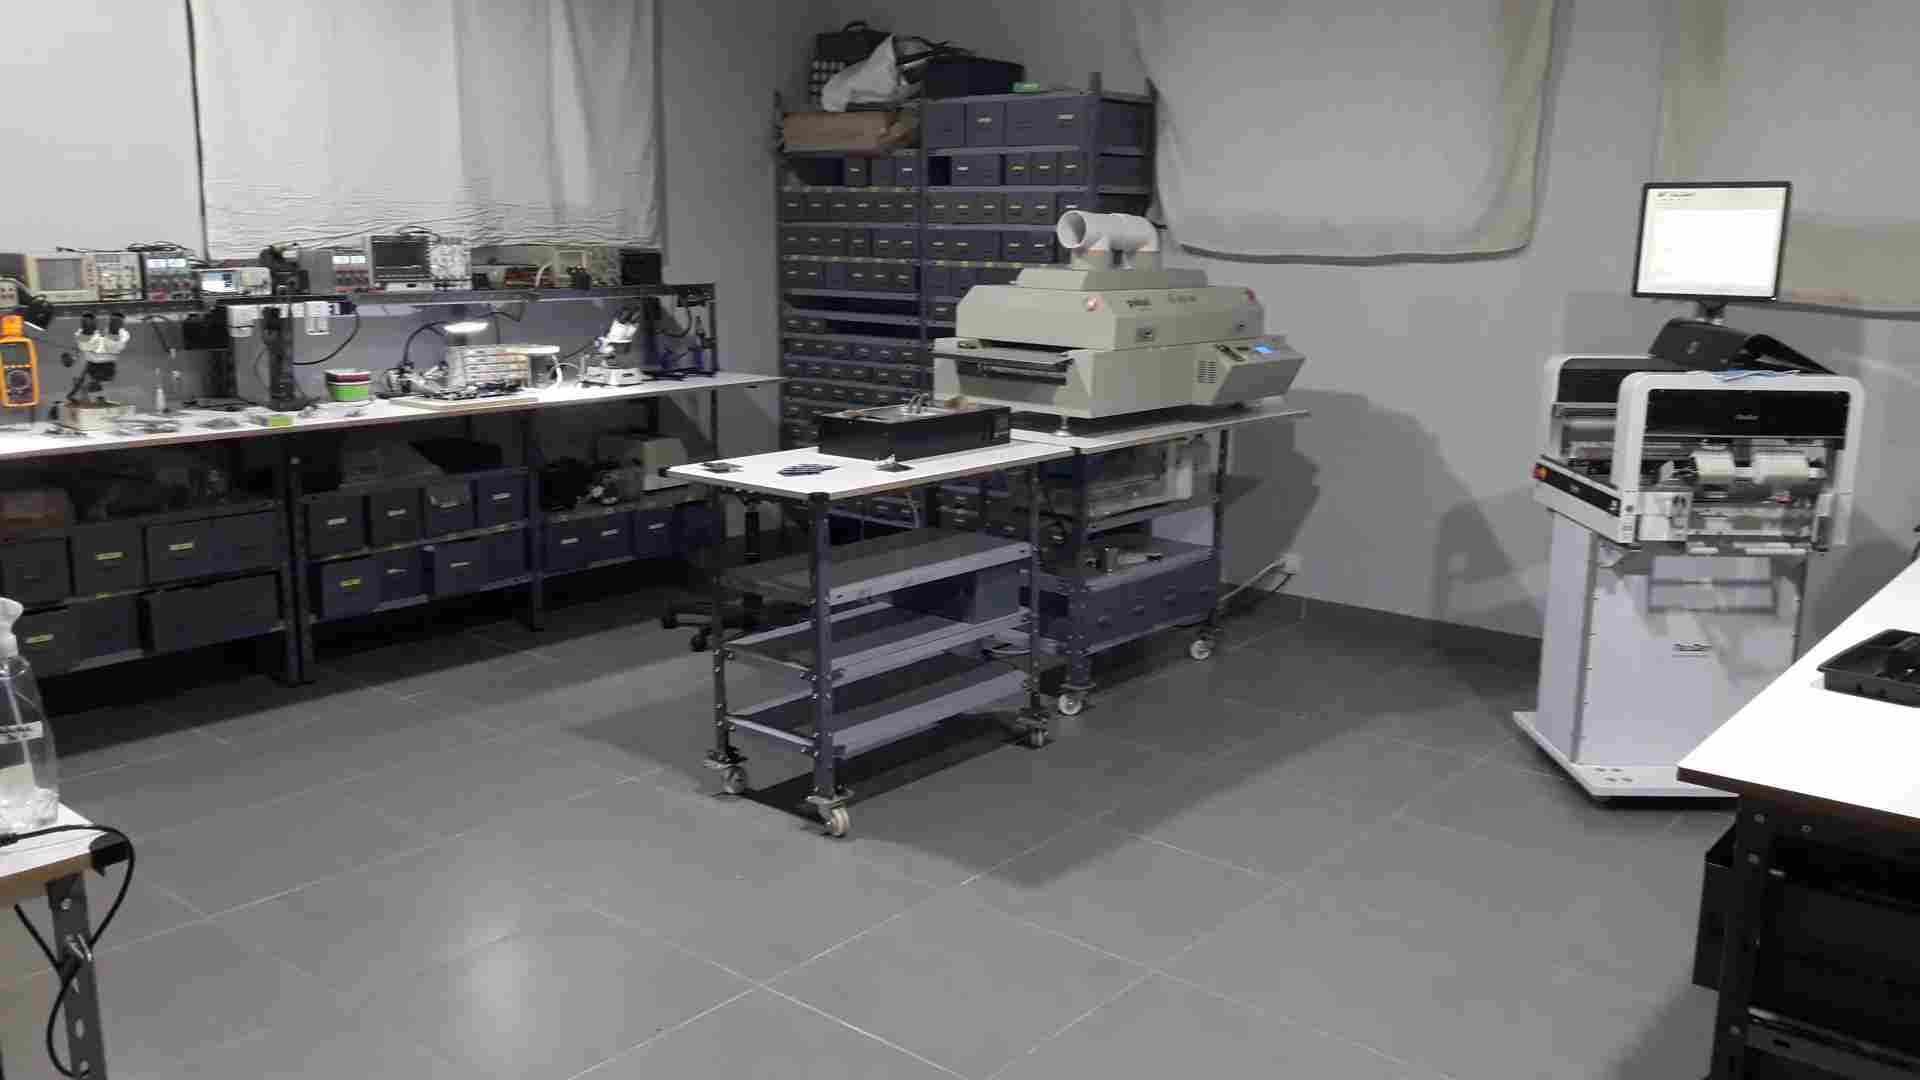
\includegraphics[width=0.3\textwidth]{ofi_dci_brc_2021_4.jpg}
%      \end{center}
%      \caption{Development lab at Bariloche, 2021. \href{\linkofidci}{Video lab. 2019}, \href{\linkofidcitwentyone}{Video lab. 2021}}
%      \label{fig:ofi_dci}
%   \end{figure}
\pagebreak
